\chapter{It's Our Future: developing methods to resist justification practices}
\label{}

\section{Introduction}
\label{}

In the previous chapter, I described my grounded theory of justification, classification and performance practices and the ways they enact capitalist realism and contribute towards the reproduction of 'vulnerability'. In this chapter, I outline my first attempt at designing to move beyond capitalist realism and resist justification practices in the form of a design project called 'It's Our Future'. In this project, I was commissioned by The Charity to create a design intervention that would help young people to think about what they wanted for their futures, and produce a manifesto that could be used to influence policymakers to work towards these futures. Despite this intent, The Charity was also focused on producing an intervention that documenting their impact and expertise. As such, one of the key design considerations of this work became how to design against justification practices. 


% According to dominant paradigms within participatory design, by taking these methods and meaningfully adapting and appropriating them to my own design and research context, I should have been able to create design interventions which enabled the people I was working with to connect with each other, build solidarities and skills, and develop powerful responses grounded in their own lived experience. As I outlined in that chapter, though, this wasn’t quite what happened. Though there were glimmers of hope, where it felt like skills, solidarities and futures were breaking through, the dominant conditioning of justification practices and the nature of subjectification under capitalist realism were stronger forces. In this chapter, I consider what comes next - what do we do when participatory design is not enough? 

I suggest that a speculative praxis is needed within participatory design in order to break past the conditioning and boundaries of capitalist subjectification. In this chapter, I detail the beginnings of this speculative praxis with reference to It’s Our Future

Both projects were based around the use of speculative and prefigurative participatory design methods that sought to both imagine new worlds and build them through their design process. I reflect on the creation and deployment of these projects and the design challenges encountered in each, before finishing with a discussion of what the kind of speculative praxis these projects means for contemporary participatory design practice.

% the limits of participatory design?

\section{Context}

In August 2019, I was primarily working with The Charity on Building Bridges, when a potential new project with them came onto the horizon. At that point entitled FutureYoungPeopleUK, The Charity was interested in running a large scale digital consultation to understand what young people wanted for their futures at a time when they felt their wants and needs had been largely overlooked. In the year prior to this, for example, there had been repeated uproar about the United Kingdom leaving the European Union (‘Brexit’). For months, there had been no significant movement on the terms of the withdrawal agreement, and when there finally was, it failed to make its way through Parliament. What followed included a Conservative Party leadership election, an illegal prorogation of Parliament, a swing towards ‘hard Brexit’ (unilaterally leaving the European Union without a trade deal) and, as we were preparing to run It’s Our Future, a general election was called. In all of this, there had been a great deal of frustration from young people – either from those who were too young to vote in the 2016 European Union membership referendum, or from those who felt the future of the country was being unfairly decided by those who wouldn’t have to deal with the consequences of it. As part of this, groups such as For our Futures’ Sake and Our Future, Our Choice were established with the backing of the People’s Vote campaign to attempt to highlight the need to consider young people’s wants and needs for the future.

The idea for FutureYoungPeopleUK came against this backdrop. Alongside a decade of austerity and a lack of prioritisation of services for children and young people in government budgets for years, The Charity were keen to run an event that brought young people’s wants for the future and being unable to influence official discourse around the future to prominence. The form of FutureYoungPeopleUK changed rapidly across the two months that we were creating it. Although its final form was It’s Our Future, a large-scale design workshop and participation event for young people to imagine and build the future, it went through a number of different iterations before this point. To explore this in full-depth, I will detail a number of key design constraints and moments of change within the overall design process, to illustrate the journey that took us toward It’s Our Future.

\section{Design constraints}

The Charity was part of a ‘civic leadership group’ composed of senior civil servants, CEOs of charities and other interested stakeholders who had become concerned about the lack of consideration of the experiences and needs of young people within civil society. In response to this, they commissioned a poll by YouGov which was responded to by 1036 young people, exploring how they felt about the future and what they felt might transform their lives if it happened in the next five years. The headlines from this work were that most young people either felt uncertain about the future or felt negatively about it, thinking that they would be worse off than they are now, and that the main things that would transform young people’s lives were money, having a better job, getting a degree, becoming healthier, and having better mental health.  The civic leadership group agreed that in the follow-on campaign work – FutureYoungPeopleUK – it was important that they did more than merely synthesize the results of this survey and communicated it to government, but instead actively attempted to ensure that the voices of young people “shaped, developed, and articulated an agenda for action, for themselves and for the country”. Their initial idea for the project centred on a two week digital conversation that we would design, facilitate and deliver, the output of which would be used to feed into the design and delivery of a launch event for a wider program of civic engagement.  In the first instance, then, our designs responded to this brief: a two-week digital conversation that could feed into the design of an in-person launch event.

\subsection{Leveraging social media and infrastructuring participation}

The Charity were keen on using a ‘snowball’ mechanism for engagement, whereby those that became involved with the project would encourage others that they knew to become involved, either by being visible through public interactions or through directly encouraging their friends to become involved. The Charity agreed to directly engage the people they supported that interacted with the YouGov survey, as a way to start the engagement with a core group of almost 100 young people. It was hoped that this core group of young people would be able to act as a ‘steering group’ of sorts, making key decisions and feeding into the overall design of the engagement.

One of our first questions, then, was which social media platform to run the engagement on. There were two key constraints here – which social media platforms young people actually use, and which social media platforms charities and other civil society actors use. Here, we conducted a rapid review of trends within social media engagement for charities and other groups that work with young people, and reflected on this within the context of the participatory social media project described in the previous chapter.  Our candidate platforms divided neatly into four categories: text-based (posts), text-based (messages), image-based, and video-based.  The platforms are shown within these categories in \ref{table:iof-social-media}.

\begin{table}[]
\begin{tabular}{lllll}
\caption{A grouping of different social media platforms by their primary functions. }
\label{table:iof-social-media}
\textbf{Text-based (posts)} & \textbf{Text-based (messages)} & \textbf{Image-based} & \textbf{Video-based} &  \\
Twitter                     & WhatsApp                       & Instagram            & YouTube              &  \\
Facebook                    & Facebook Messenger             & Snapchat             & TikTok               &  \\
                            & Discord                        &                      & Twitch               &
\end{tabular}
\end{table}

At this stage, several platforms were eliminated for their potential irrelevance and for some technological limitations. We disregarded Facebook and Facebook Messenger, for example, for their relative lack of youth users – informed by the participatory social media project from the previous chapter. We also disregarded Snapchat at this stage because of the insights from that work that organisations using Snapchat felt “unprofessional” to the young people we conducted the work with. Though Twitter also has a low youth userbase, we decided to include it because it is the primary social media of many charities and so we felt it would be useful for raising the profile of the engagement to other charities. We also disregarded Twitch at this stage, as although it has a large amount of young users, only a very small percentage of users have high viewerships, with the majority of users on the platform being viewed by only one or two people. In particular, frequently-visited channels on Twitch tend to have built their audiences from multiple hours-long streams at a time, something we would have been unable to do due to time constraints. Finally, we eliminated WhatsApp from our list of potential platforms as we wanted to potentially automate aspects of the structure of the engagement and at the time WhatsApp’s API was still in beta testing. 

This left us with five candidate platforms – Twitter, Discord, Instagram, YouTube and TikTok. Rather than choosing to focus on just one of these, at this stage we decided to develop a strategy for infrastructuring participation across social media platforms. At this stage, our plan was to design and develop the content for the engagement and automate posting it across each social media platform through the use of multiple bots, which would deliver the content across each day of the engagement. We decided, then, that our central social media platforms for the engagement would be Instagram, Twitter and Discord, and that YouTube and TikTok would act as potential amplifiers for the engagement if we could enlist the support of some prominent YouTubers and TikTok accounts. The technological side of the ‘snowball’ strategy, then, became to have a two-phased engagement: one where anyone could potentially become involved by seeing a post on Instagram or Twitter and respond to it, and to attempt to convert as many people as possible to participating more significantly within the project by having a bot respond to social media engagements with replies that developed a young person’s ideas and invited them to join the organising group, hosted on Discord. 
	
Based on my previous research, the insights of a number of youth workers throughout my research, and the insistence of The Charity, we felt that it was important for the initial engagement within the project to hinge upon asking the simplest, clearest question possible. Although we were not using an explicit model of participation within this, our central idea was that asking questions about one’s own lived experience makes for a question that is clear and simple to ask. We set about trying to find the simplest possible question that asked what participants wanted for the future but that was grounded in their lived experiences. Initially, we began with:
	
What changes would you make to the country now so that you can live your best life in 3 years?

We then created a version of this that had two options for participation, one which was the lowest barrier possible, and one which required a medium amount of effort:

How do you feel about the UK at the moment? DM us an emoji, a story or a reaction. (low)

How do you feel about the UK at the moment? DM with what you would change. (medium)

At this point we were trying to understand how we could make this even simpler whilst also diversifying content across each of the five substantive areas of the YouGov survey. We decided that this would dilute the ask of the project, potentially confusing participants, and so we settled on boiling this down to a single ask again, unified for each content area:

Make something – whether a song, poem, drawing, video, etc. – about how you see your future. 

This would have been the final version of the ask for the project – at this point entitled \#MakeYourFuture – if we had not had to contend with the different ways that justification practices then invaded the project and changed our parameters. 

\subsection{Navigating justification practices}

After the ways that justification practices impacted the Life Story Work film, I perhaps should have anticipated the ways that they began to take root in the nascent #MakeYourFuture project.  Ultimately, having to navigate the way that justification practices played out in this context changed the nature of the project considerably, moving it from a digital engagement to a physical participation event/design workshop. They also reveal more about the ways that justification practices can shift and adapt to new circumstances, especially if those circumstances might present a new way of operating. 

Despite The Charity approaching us for the project, we were required to visit The Charity’s head offices in London to pitch our version of the project (excerpts from the pitch slides can be seen in figure x). The version that we pitched reflected the project as it has been explored so far – a two-phase interaction, conducted across multiple social media platforms, rolling into a core organizing group of around 100 young people hosted on Discord. Between the two phases, we would do follow-up engagement with participants in order to help them flesh out their ideas and proposals for the future and politicize the issues that they saw as key to a future. When we presented this to The Charity, their central concerns were around safeguarding and ensuring that we could ensure the safety of all of the young people involved in the project. 

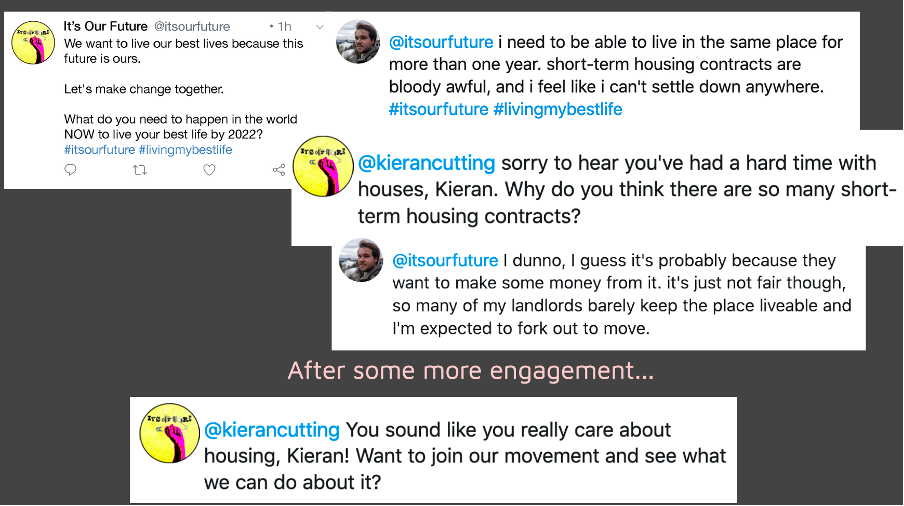
\includegraphics[]{Images/7/iof-1.png}
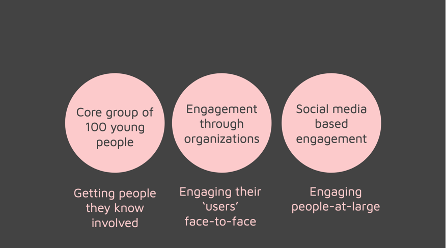
\includegraphics[]{Images/7/iof-2.png}
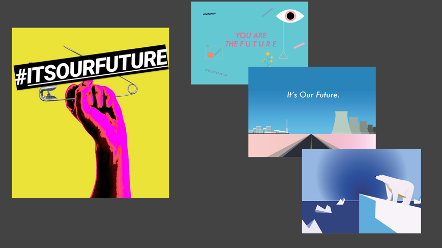
\includegraphics[]{Images/7/iof-3.png}


Of course, we were also concerned with the safety of young people within the project – both from a legalistic perspective and a moralistic one that we wanted to ensure we create safe, healthy and healing spaces for young people to exist within. Discussion quickly fixated on the use of specific digital technologies within the project instead, and the degree to which they were perceived to be ‘safe’ or whether they might cause problems for the organization if they were seen to be associated with them. In the months prior to the pitch meeting, for example, The Charity had campaigned against TikTok for the ways it felt that it put young people at risk of sexual exploitation (due to the ability for anyone to livestream from it). A large part of conversation on the day then focused on whether TikTok was a viable platform for The Charity to be associated with given this campaign. They were adamant that it could cause themn reputational damage to be seen to go against their previous campaigning and made us ensure that we wouldn’t use the platform as part of the project.

Similarly, a large amount of discussion focused on the use of Discord. The majority of the members of the team had never heard of Discord or only had passing familiarity with it, so we had to describe its functions in depth. It is worth noting here that at the outset of the project, The Charity had promised us a dedicated member of staff to deal with safeguarding concerns during the project, which we had made a condition of our engagement, as we did not have the requisite safeguarding experience within our team to manage this.  As such, we felt that we were creating a safe space on Discord, that only specific young people would be invited into, conversation would be monitored and moderated in case any concerning disclosures were made or worrying behaviours were exhibited, and that a dedicated member of staff would be on hand to deal with any legal safeguarding issues that occurred. Discussion fell to the procedural aspects of using a platform like Discord – did The Charity have a risk assessment for it? What did their head of Digital think of it? Could young people contact each other through it? Who would be on the platform?

It would be easy to see The Charity’s concern around safeguarding here in good faith – that they are an organisation that advances the cause of the rights and safety of children and young people and thus want to ensure that they can create and maintain safe spaces for them. Yet it became clear throughout what followed that the primary concern of The Charity were focused on compliance, their reputation, and other values that emerged from a context saturated with justification practices. Their concerns were less about protecting children and young people (though I do not doubt that they did actually care about this too) but instead protecting their reputation as a charity that occupies a central role in public influencing around the delivery of support services to children and young people. This even influenced the creation of the event and engagement in the first place – centrally, The Charity hoped to have a high-profile digitally-anchored event that would enable them to position themselves as digitally innovative, excellent at partnership-working, and as the main guardian of the voices and experiences of children and young people.

In It’s Our Future, I was more attuned to the ways that justification practices could affect design processes but I had yet to learn the full scale of what they could affect and try to change. As such, at this point I knew we were experiencing justification practices playing out but I did not yet quite know how to resist them. I found myself beginning to bend to The Charity’s wants and needs, unable to fully hold my own against people whose entire job is influencing. At first, then, we set about trying to reassure The Charity that everything would be fine – that we would be able to control and moderate interactions, ensuring nothing ‘bad’ or unintended would happen. We had fallen prey to justification practices ourselves – willing to use digital technology to enact a politics of control and classification. We set about creating an in-depth process diagram of the entire project to explain our logic (pictured in figure x) and to highlight interaction touchpoints so that The Charity would be sure that we could triage any potentially concerning disclosures to them, and that we would otherwise be monitoring the chat fairly constantly.

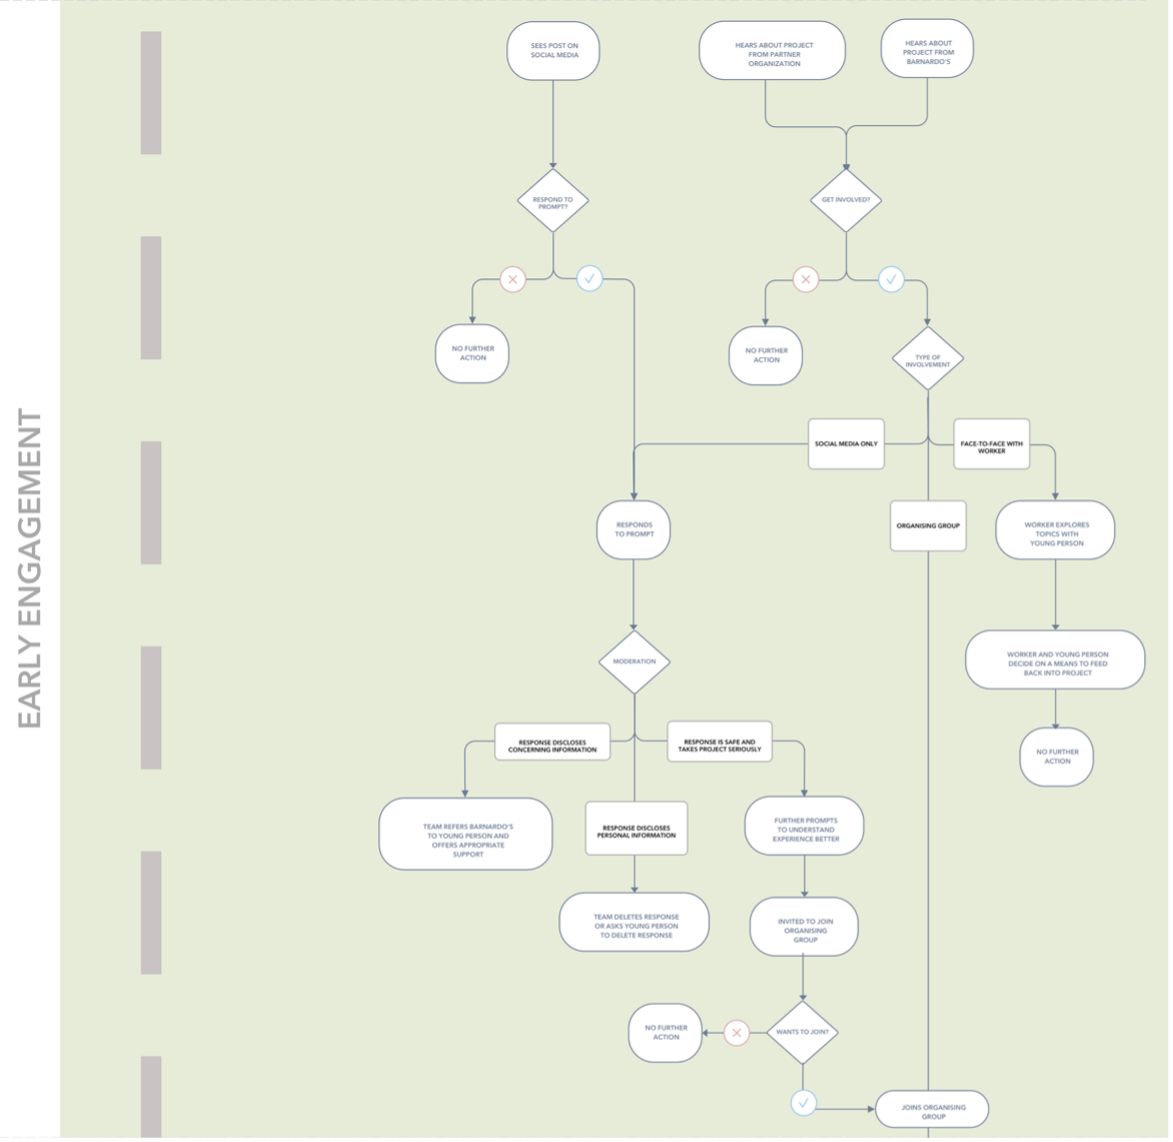
\includegraphics[]{Images/7/iof-process-1.png}
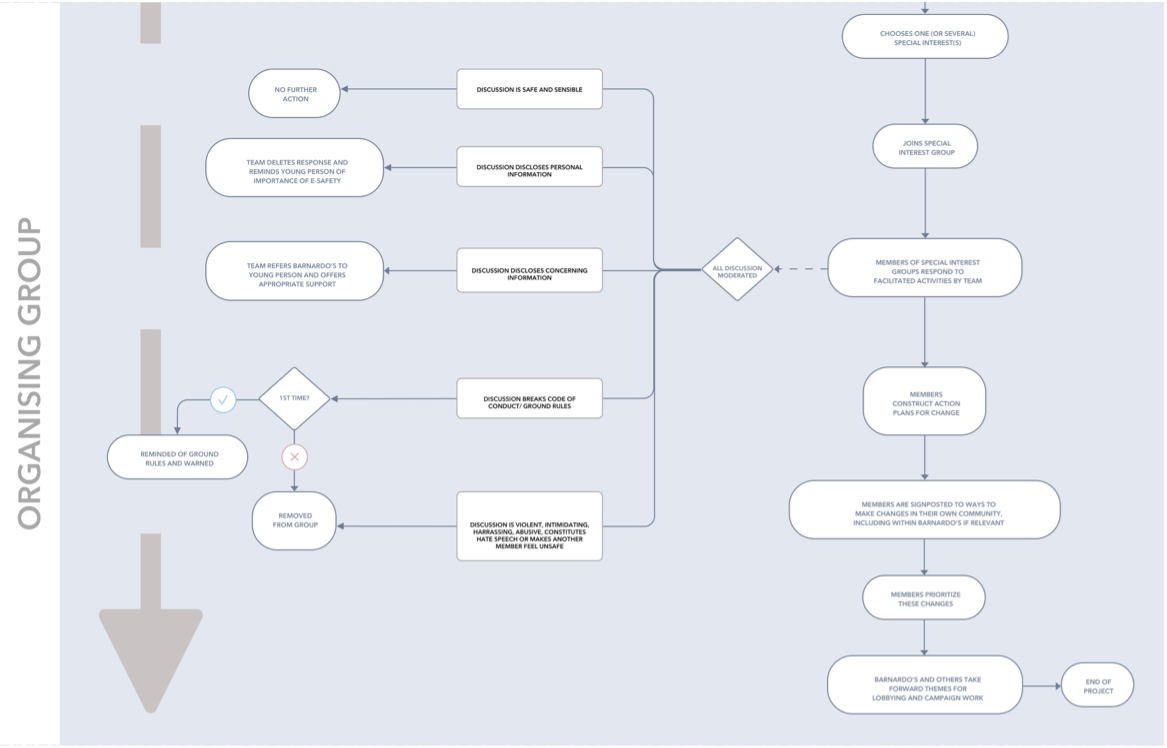
\includegraphics[]{Images/7/iof-process-2.png}

Justification practices always have a human cost, and I can briefly explore this in a way I perhaps have been unable to elsewhere in the thesis as I was the perpetuator of them and affected by them. At this time, The Charity had created an environment of artificial scarcity. They had contacted us with less than two months to go until their intended end of the project/launch for a wider aspect of engagement, and then set on making it seem as if we weren’t acting quick enough. I found myself having to jump between roles to attempt to satisfy The Charity’s increasingly large demands. I had to play project manager, interaction designer, service designer, researcher, youth worker, and safeguarding lead. I had to constantly switch between all of these roles, beginning to wonder what the right place for me in all of this was. The work began to creep into my personal life – I was working later and longer hours, which came to a head when, after the pitch meeting, I went on holiday with my parents and brother. We were meant to have a relaxing week in North Wales, spending time together where we hadn’t seen much of each other. Yet I found myself making the process diagram in figure x in the back of my dad’s car in Llandudno whilst the rest of my family got ice creams. My stress levels were rising more each day, and I was unable to get the benefit of what was meant to be a rejuvenating time away. I came back to my PhD the week after having spent hours on holiday doing work on It’s Our Future in order to meet The Charity’s increasing demands, with no offer of reciprocation on their side. The project had started on a grounds of mutual collaboration, but at this point it was only myself and a few other members of the design team doing anything.

As we began to develop the visual direction of the project, moving at a speed that was necessary in order to get the project launched on the intended date, we faced increasing resistance. Though we had previously agreed that the image of a solidarity fist was perfectly fine to use within the project as one of our intentions was creating a protest-like movement for young people, once we presented The Charity with materials that included a solidarity-fist in the logo, we were met with pushback. They felt that the logo “look[ed] uncomfortably close to a fist and that is obviously not what we or you are about…”, inviting us to think of “another arresting image which couldn’t be misinterpreted in that way?”. Then they were concerned that It’s Our Future was too generic, wanting the name instead to be the similarly generic OurFutureOurUK in order to make it “more upfront that this is seeking input and energy from across all four corners of the country plus… appropriating a term in ‘UK’ that too often gets used/abused by extreme right wing, it’s our nation not theirs”. In essence, The Charity wanted to strip any conception of the political from the project – framed through the language of being ‘concerned’ – and ensure that the project made reference to the national stretch of the project in order to maximize their own potential acclaim, highlighting themselves as national influencers and the legitimate voice of children and young people.

Figure x. An earlier logo design for It’s Our Future. 


We were still towing the line with The Charity at this point – although we were uncomfortable with using their choice of name as we felt it perpetuated rather than appropriated the use of ‘UK’ rather than the extreme right wing. As such, we decided to settle the discussion by creating a new logo which emphasized the UK within it and disposed of the solidarity fist.   This logo (pictured in figure x) was still met with further pushback, as The Charity were concerned that “the ‘hashtag’ obscures too much of Wales”. Although we moved the title (and changed the colouring of the Republic of Ireland, so as to make clear it was not included within the scope of the project, as we anticipated this being a further comment if we didn’t change it), we were becoming tired of the level of granularity at which concerns were being raised, as we felt they did nothing to develop the work but instead just served the needs of bureaucratic justification practices. After this, an email arrived which made us put the brakes on the project as it currently was, in which [Stephen], the lead on the project from The Charity’s side, asked us if we could share answers to the following:
	
•	Our safeguarding policies
•	Any learning picked up from safeguarding challenges throughout research conducted by Open Lab 
•	Whether we could take responsibility for any agencies we contacted to comply with our safeguarding policy
•	Whether we could make explicit in promotional materials that the project was not the place for highly personal disclosures
•	An age-verification process in the Discord phase of engagement 

We were floored by the level of detail that they wanted, and I was struck by a sense that I could not (legally!) make these kinds of decisions or answer these questions. 

Figure x. The final “It’s Our Future” logo.

As a team, we had to go through a design process just to respond to the email.  I drafted an initial reply – incredibly lengthy, perhaps too direct in tone, putting a stop to the entire project. The level of engagement from The Charity that we had seen thus far was so minimal that we had been working in the dark, unable to make any meaningful decisions but with a huge amount of pressure on us to deliver the project on time.  We sent an email outlining our inability to take on the responsibilities that they wanted us to, the lack of sufficient reason under GDPR to hold the kinds of data they wanted us to, and our inability to support an age-verification process within the Discord engagement. [Stephen] replied, and the plug was pulled on the project – in its current form. 

\subsection{Towards It's Our Future - the event}

With the additional burdens that The Charity kept placing onto us as a project team, and their asking us to commit to things that we legally didn’t think we were able to on behalf of the university made us take a step and realise just how far we had come from the original intention of the project. We had wanted to see if we could use this project as an attempt to understand how one might infrastructure participation across multiple different social media platforms and politicise issues that emerged from people’s lived experiences, helping them to connect them to wider concerns. In this sense, the core aim of the project for us was about identifying ways to intentionally do digital movement-building, building on the critical pedagogical work from the Life Story Work project. In understanding how we might approach It’s Our Future in a purely physical, design workshop-led sense, this became our new anchor. 

We revisited the original project idea. When we began, we intended to use multiple social media platforms and bots across them to ask a simple question of young people. In its final form, this question was “What would genuinely transform your life if it happened in the next 5 years?” We would put this out across the social media platforms each day, hoping that as more people interacted with the posts, more people would find the account and interact with it. In order to move people from the ‘light’ participation of responding to a tweet to the more involved interaction of being involved in an organising group, we planned to develop a bot that would respond to engagements with the intent of contextualising the issue, politicising the issue, or building a critical consciousness around that issue. Our ideal interactions would have been something akin to figure x. We used the idea of taking a simple ask and contextualising, politicising, and building critical consciousness around it as our starting point as the physical version of It’s Our Future. 

As we had conducted a rapid review of current best practice around social media-based engagement for the digital version of It’s Our Future, we similarly set about conducting a rapid review of evidence around protest and activist movements across recent history, and explored movement-building methods. Although our historical review was useful, it provided no clear anchors that we used in the workshop itself. From this review, three central concepts became clear that we used as anchors throughout the rest of It’s Our Future – counterpower, emergent strategy, and research justice. We threaded the ideas of these three concepts throughout It’s Our Future and they became part of the DNA of what we were trying to achieve through the workshop. 

We drew from Tim Gee’s work on counterpower [ref] as we felt this matched our current understanding of the contemporary political situation. As explored in chapter 2, the contemporary political moment of this research is one marked by a stagnant neoliberalism as it gives way to a violent, excessive fascism, and both of these forces combine to create a hegemonic politics of capitalist realism that attempts to resist any attempt to change it. The plasticity and reconfigurability of capitalist realism means that attempts to resist are often absorbed into the fabric of capitalism itself and then redeployed as a site of potential accumulation. Take, for instance, Audre Lorde’s notion of self-care as an act of “self-preservation… [and] political warfare” [ref]. This came from Lorde’s understanding that to care for one’s body as a Black woman is to attend to one’s self in a way that the state and society at large never will; it is to create a container of rest, recovery and healing that is essential to overthrowing the dominant paradigms that perpetuate injustice. In recent years, we have seen this colonised and made a site of accumulation and commodification through the sale of “self-care” products, particularly by ‘wellness’ or ‘holistic living’ brands who use spirituality as a unique selling point. To resist capitalist realism, then, requires the formation of a counterpower within those who are not afforded power by the dominant structures of late stage neoliberal capitalism. 
	
In Tim Gee’s book [ref], he identifies four key aspects to building counterpower – consciousness, co-ordination, confrontation, and consolidation. Consciousness roughly corresponds to the level of problem-articulation and building critical consciousness that I have already explored elsewhere – this is understanding that there is a problem and creating the conditions for counterpower to be built. Co-ordination is the stage of building counterpower through a movement to address that problem. Confrontation is the moment of confronting those with traditional power, challenging their power with the movement’s own counterpower. Finally consolidation is about maintaining counterpower after it has been used to confront the oppressor, continuing to hold power and ensuring that turns into real and material change. We used these stages as footholds that we felt the It’s Our Future process should be designed around. Effectively, this meant that throughout It’s Our Future, there must be a clear mechanism for articulating problems, building power, confronting those with traditional power, and maintaining power. 

The work of adrienne maree brown was (and is) the most transformative aspect of the work from It’s Our Future, as it taught us a number of foundational concepts around movement-building work that guided the methods we developed to use to build counterpower within the workshop. Her concept of emergent strategy is developed from the fiction work of Octavia E. Butler and the characters within her Earthseed series as they attempt to build new worlds in the shell of the old to ensure they might be able to survive and thrive.  There are several core aspects to emergent strategy.  [fill them in here] Our key takeaway from the work of emergent strategy was to expand ideas within the stage of critical consciousness development (i.e. to not get too focused on specifics, but to explore alternatives at the same time), to envision collective futures that everyone involved actually wants to work towards building, to build trust between members of the group so that they can build strong relationships which support them throughout the social change they wish to make, to decenter individual leadership and instead build in as many opportunities for decentralised leadership and fractal expressions of agency, and to accept change and work with it, rather than tightly planning every single aspect of something. Within the frame of counterpower, emergent strategy provided some of the connective tissue. 

Finally, we used the ideas of research justice to… they gave us a clearer understanding of ways that we could equitably structure our research and design processes, and the ways that we could center the material needs of those with lived experience of oppression or trauma, and… Our encounter with research justice made us reconsider the way that our positionalities and the positionalities of the civic leaders and frontline workers might affect any engagement within the workshop. In particular, research justice made us think about the kinds of knowledges that we center through our academic knowledge-making practices, and we attempted to create It’s Our Future as a space where situated sense-making and collective understanding were valued more than the attempted creation of any kind of pseudo-objective knowledge. 
	
The design space for the physical It’s Our Future event, then, centered on:

•	Having a simple ask, that could be answered from the frame of one’s own lived experience,
•	Building critical consciousness, to help transform this simple ask into a much clearer articulation of the political and social problems that underpinned that experience,
•	Building counterpower in multiple ways, through the exchange of skills and resources,
•	Ensuring the overall process centered on building trusting relationships,
•	Ensuring that imagining and meaningfully inhabiting collective potential futures was at the heart of the experience,
•	Emphasizing the ability of all present to make material changes, at different scales,
•	Providing opportunities to safely confront oppression,
•	Leveraging situated sense-making to avoid the presentation of pseudo-objective knowledge,
•	Of course, avoiding justification practices taking root wherever possible. 

Having determined the design space for the physical event, we set about creating a process and mechanism that met as many of our criteria as possible as well as possible. When it finally took place, then, the It’s Our Future event focused on groups of young people playing a card game with each other, civic leaders, frontline workers, and facilitators, to imagine and build futures which respond to what they felt would transform their life if it happened.  

\section{It’s Our Future: the card game}

The It’s Our Future card game was split into four parts which anchored our design workshop and participation event. These four parts were:

1.	What would transform your life?
2.	How are things now?
3.	Dreaming the future
4.	Building the future

The central mechanism we used throughout the It’s Our Future card game were three kinds of cards – idea cards, prompt cards, and summary cards (pictured in figure x). Each of these were marked with a different colour to make their different purpose clear. The blue idea cards were designed to be the central unit of interaction throughout the workshop, used almost like post-it notes would be in many design workshops – they were the central place that people would write their ideas, no matter how well developed. The pink prompt cards were for external prompts – as in the icebreaker activity or in part 3, dreaming the future, where participants were invited to reflect on what a potential future would be like in a given scenario. Finally, the black summary cards acted as a point of synthesis, used primarily at the end of each part of the day to ensure there was a coherent collective point of sense-making – and pragmatically ensuring we weren’t dealing with tens of cards at a time. Alongside these cards, the final activity of the day also used blueprint cards, roughly A5 sized cards that enabled people to create a final point of synthesis for themselves which they would take away and have as a reminder of their commitment to action (pictured in figure x). 

Figure x. The It’s Our Future idea cards, prompt cards, and summary cards.

Figure x. The It’s Our Future blueprint cards. 

The basic intention of the activities of the day was to create a fun way to collectively imagine futures, build relationships between participants, identify future actions and then find ways to make those happen. The first activity, ‘what would transform your life?’, was framed around our ‘simple ask’ from the digital engagement -  ‘what would genuinely transform your life if it happened in the next 5 years?’. After icebreaker activities to help the group to get to know each other and set some ground rules for engagement, participants were invited to write on three blank cards something that would completely transform their lives if it happened in the next five years. These cards were collected, shuffled, and dealt back out to them. Taking it in turns, they could then play the ‘game’. On their turn, if they had cards in their hand, they could:

•	Play a card, explaining why someone might think that would change their life, or
•	Connect a card, explaining why the two issues they are connecting are related.

If they didn’t have cards in their hand on their turn (i.e. they had played all of their cards), then they could either:
•	Connect a card, explaining why the two issues they are conncecting are related, or
•	Discard a card, explaining why it’s less related to the other ones.

When participants decided they were happy with the cluster on the table – and they had gone an entire round with no participant wanting to change any aspect of the clusters – they had formed their priority (or priorities) for the day. The cards were designed to encourage this connecting behaviour, with the edge of each card featuring semi-circles so that when they were joined to another card they formed a complete circle. By grounding the activity in a simple ask, we ensured the lowest possible barrier to participation, which we created a safe container for by ensuring that participants’ responses were anonymous. By then shuffling and re-dealing the cards and making the mechanisms of the ‘game’ be built around explaining why issues were related or important, the ‘game’ built solidarities between participants as they knew that each card represented an issue that was important to someone at their table. It also served the pragmatic function of identifying shared concerns of a group that had never met before.  

In the next activity, ‘how are things now?’, participants took the shared issues they identified in the previous activity and were invited to summarise these onto a summary card. In doing so, we hoped to encourage groups to collectively make sense of their experiences – rather than be told what their issues to focus on were – and meant that the summary cards could be the focus of further interaction, rather than a huge number of individual cards. Once groups had summarised their issue(s), they were invited to think about a possible past – thinking backwards from each of these issues, which acted as problem statements, to potentially identify who or what might have been involved in making things the way they are right now. For example, if a group’s concerns centered on climate change, then this activity would ask how the world might have arrived at a situation in which anthropogenic climate change was a threat to their futures, who might have been involved, and what they might have done. This activity was based in trying to get participants to be able to map out the actors and factors involved in the thing that they wanted to change, to give the futures that they would imagine in the next activity a material basis to arise from. To return to the climate change example, this might support the group to think about the people with a vested interest in the continuation of the mass use of fossil fuels and as such also acts in a critical pedagogical sense, helping young people to think through their issues with a lens of critical consciousness. 

The third activity was called ‘dreaming the future’. In this activity, participants were presented with everyday activities on prompt cards. These activities were add them here, and participants were asked how these activities might be different in a world which had made the changes that they wanted for the future. The idea of this activity was to articulate a shared vision of the future and to help our participants to meaningfully occupy the space and feeling of the future – to richly flesh out that future world and to make it seem practically possible. Participants were encouraged to pick one or a few of the changes synthesized onto summary cards and to think about how the prompt cards might be different in light of these. To return to the climate change example, it might be that in a world which isn’t threatened with an active climate apocalypse, going to the cinema requires getting there in a form of public transport powered by renewable energy. 

Finally, the last activity, ‘building the future’, was based in getting participants to make the connections between their imagined future and what that felt like, and their experiences in the present. It was intended to help them to think of the practical changes they could personally make to get closer to that world. As groups were composed of young people, frontline workers, and civic leaders, this activity was informed by a variety of identities and positionalities. Participants then wrote these actions on ‘Blueprint for the Future’ cards and took these home with them as a reminder of their commitment to continued action. This activity was intended to synthesize all previous activities (as pictured in figure x) – activity two could be placed on the left hand side, activity three could be place on the right hand side, activity one could be roughly in the middle and the content of this last activity would fill the space between activities one and three. 

It was our hope that the sum total of all of these activities, combined with The Charity’s plans for follow-up engagement, would lead to the beginning of some critical political engagement. This was especially pertinent as just prior to It’s Our Future taking place, a General Election was called in the UK. The events of It’s Our Future thus took on a new parliamentary political importance – and, as I will explore later – let to new challenges from the ways in which The Charity hoped to use the engagement as part of their policy and influencing strategy. 

\section{How It’s Our Future worked in practice: an analysis of the methods}

\section{The It’s Our Future manifesto}

As It’s Our Future now happened against a backdrop of a General Election, The Charity were both keener than ever to use It’s Our Future as the basis of an influencing strategy, and simultaneously reluctant to commit to anything which might be considered overly political and violate electoral rules around charity campaigning (the so-called ‘gagging law’). As agreed beforehand, we set about doing a thematic analysis of the data from It’s Our Future in order to reflect the discussions and proposals that came through on the day, which The Charity had planned to take to prospective MPs and encourage them to sign up to these pledges. We then adapted this into a manifesto format, which we felt was consistent with the vision and aspirations of the event (pictured in figure x). 

Figure x. A screengrab of the It’s Our Future manifesto. 

The data from the event itself – the content of the young people that we worked with’s futures – focused on six key themes. These themes were ‘Let us use our power’, ‘Support our mental health and wellbeing’, ‘Education that works for everyone’, ‘Building communities and opportunities’, ‘Technology that works for us’, and ‘Action on climate change, now’. In what follows, we will briefly explore each of these themes in order to do justice to the richly detailed proposals that young people developed through participating in It’s Our Future.

In ‘Let us use our power’, young people discussed

In ‘Support our mental health and wellbeing, young people discussed

In ‘Education that works for everyone’, young people discussed

In ‘Building communities and opportunities’, young people discussed

In ‘Technology that works for us’, young people discussed

In ‘Action on climate change, now’, young people discussed

\section{The return of justification practices}

Things began badly when it came to the follow-up engagement. After we had prepared an almost-final draft of the manifesto with them, they shared it online without ever notifying us, and began their own program of engagement. We had intended to run a parallel program of engagement, so that we could maximize the impact of the research and ensure that young people’s wants for the future could get as much traction as possible, but with The Charity launching without us we had started on the backfoot. We attempted to do some engagement, but by that point it was too late into the General Election to meaningfully influence candidates and our window of opportunity had closed. 

Towards the end of the manifesto creation process, we repeatedly went back and forth with senior members of The Charity’s team to fight over individual word choices. It felt as if I was seeing the full force of justification practices in action, as [Debbie] repeatedly tried to convince me to misrepresent the research we had conducted and change the word ‘power’ to ‘voice’, because it was a more ‘politically savvy’ word to use. Although we managed to stay true to the research and hold back the forces of control and classification, it felt that perhaps the cost we had paid was losing The Charity’s interest. When we first created the manifesto, The Charity were keen to do more work with us on the manifesto, saying that we should talk to their board of trustees about the work, that we could pilot follow up small-scale engagements with various of their services, and so on. This slowly seemed to disappear. The election was over, then it was Christmas, then the New Year. At this stage, I had given up any hope of further engagement with The Charity on It’s Our Future at the very least, and had turned our attention back to our work with Small Steps and Building Bridges, hoping to refine the methods we used in It’s Our Future in these different contexts – closing the loop of my research, so to speak, by taking the learning of It’s Our Future back to them. 

At this time, I created a document called Design Strategies against Justification Practices (pictured in figure x) where I had attempted to distil my thinking around the use of the It’s Our Future methods in other contexts. In it, I split these methods and approaches into three areas – identifying problems, making alternatives, and principles. In the identifying problems area, the methods were ‘sharing experiences’, ‘group forming’, ‘problematizing’, and ‘connecting experiences’. In making alternatives, the methods were ‘deconstruction’, ‘defamiliarization’, ‘envisioning’, and ‘building’. Finally, in ‘principles’, there were ‘pedagogies’, ‘playfulness’, ‘situated sensemaking’, and ‘healing’. These principles were parameters through which the other methods should participate. For example, you cannot just have a group-forming method to act against justification practices in design processes. Instead, you must have a group-forming method which is also healing, or is also pedagogical, for example. 

Figure x. A few pages from Design Strategies against Justification Practices. 

The Design Strategies against Justification Practices represented the synthesis of the It’s Our Future work and was the basis of the work I had hoped to do with Small Steps and Building Bridges in the summer of 2020. In March 2020, we were preparing to get the It’s Our Future manifesto printed in preparation for some follow-up engagement. The day that we were ready to go to print, we got a call saying that only essential purchases were being approved. Sadly, in March 2020 much more important things were happening than It’s Our Future’s manifesto being printed. In March 2020, the United Kingdom went into a state of lockdown due to the novel coronavirus COVID-19, and as a global pandemic took hold, people were separated from each other, plans for the future were disrupted and millions died.  The research I had planned up until this point was not spared – both Small Steps and Building Bridges had more active concerns with supporting the care-experienced young people they work with, whilst also modelling the importance of taking the restrictions around the coronavirus seriously. It’s Our Future was no more. 

% something 